\section{Teste de Aderência}

De acordo com \citeonline{oliveira}, a grande dificuldade com o desenvolvimento de modelos hidrológicos é a validação dos resultados obtidos, onde se deseja determinar indícios documentados que provêm um alto grau de garantia a um processo específico, assegurando constantemente que os resultados estejam de acordo com a distribuição presentada para o conjunto de dados.

Diversos procedimentos estatísticos convencionais têm sido usados para este fim, tais como teste de comparação de médias (teste t), testes de comparação de variâncias (desvio padrão) como teste F, intervalos de confiança e outros diferentes níveis de probabilidade, e para a comparação de frequências de dados agrupados são normalmente utilizados os testes $\chi^2$ e Kolmogorov-Smirnov \cite{oliveira}.

O mesmo autor afirma que quando se ajusta uma distribuição de probabilidade a um conjunto de dados, trabalha- se com a hipótese de que a distribuição representa adequadamente aquele conjunto de informações.

Assim, \citeonline{climatologia}, comentam que em trabalhos de hidrologia, para se julgar a adequação do ajustamento dos dados observados a distribuição de frequência os testes estatísticos qui- quadrado ($\chi^2$) e o de Kolmogorov- Smirnov tem apresentado os melhores resultados.

\subsection{Papel de Probabilidade}

O papel de probabilidade é uma técnica gráfica utilizada para verificar a adequação dos dados a um determinado modelo estatístico \cite{papel}.

O papel de distribuição normal é escolhido quando os dados são simétricos à esquerda e à direita da média. O papel permite valores positivos e negativos e é adequado para muitos tipos de dados, por exemplo, dimensões de partes estruturais, cargas médias pontuais no tempo, níveis de água, etc. O papel de distribuição Log-Normal é escolhido para dados em que não existem valores negativos. Podendo ser utilizado em resistências de materiais, cobrimento do concreto, intensidade de chuva, vazão. \cite{papel}.

Cada valor de uma amostra é representado por um ponto em um dos papeis de probabilidade escolhido. \citeonline{papel} define as seguintes etapas para obter os pares coordenadas que serão inseridos no papel de probabilidade.

\begin{enumerate}
    \item É criada uma tabela com os valores em ordem decrescentes.
    \item Cada valor é associado, a sua correspondente posição n, de um total N valores 
        \begin{equation}
            F_x(x_n) = \frac{n}{N+1}
        \end{equation}
    \item Cada valor $x_n$ da amostra é plotado no gráfico como um ponto $(x_n,F_X(x_n))$ sobre o papel de probabilidade
\end{enumerate}

A série de pontos obtidos é aproximada visualmente usando a reta mais apropriada. Se os valores extremos da distribuição são de interesse, então, mais peso deve ser dado a eles. Se fortes desvios forem observados, talvez mudar o tipo de papel de probabilidade ajudará. O procedimento é repetido até que uma aproximação satisfatória seja obtida \cite{papel}.

Existem programas de computação que fazem esse trabalho, dando peso igual a cada um dos pontos de dados. Deve-se afirmar, no entanto, que alguns problemas exigem maior ênfase nos menores valores, alguns nos valores maiores. A reta escolhida, juntamente com o tipo de papel de probabilidade, caracteriza a distribuição apropriada \cite{papel}.

\subsection{Qui-Quadrado}

O teste do $\chi^2$ é aplicado para verificar o ajuste de distribuição de probabilidade conhecida, no caso a gama, a uma amostra de dados de uma distribuição de probabilidade desconhecida. No teste do $\chi^2$ , a hipótese de nulidade admite que as frequências observadas se ajustem as frequências calculadas com a distribuição teórica (gama, exponencial, normal, Weibull) com seus parâmetros estimados com base nos dados amostrais. O valor de $\chi^2$ é dado pela Equação \ref{eq:chiquadrado}.

\begin{equation}[h]
\label{eq:chiquadrado}
    \chi^2=\sum_{i=1}^{k} \frac{(F_{0i}-F_{ei})^2}{F_{ei}}
\end{equation}

Se o valor do $\chi^2$  calculado é menor que o $\chi^2_{1 - a, k- p - 1}$ , sendo esse último proveniente de uma distribuição com GL = k – p - 1 graus de liberdade, sendo p o número de parâmetros estimados com base nos dados (p = 2, para o caso da distribuição gama) e a é o nível de significância estabelecido à hipótese de nulidade não é rejeitada e pode-se afirmar que os dados amostrais se aderem à distribuição teórica com um nível de significância a. A Figura \ref{fig:qui-quadrado} mostra as duas zonas, de aceitação e rejeição do teste $\chi^2$.

\citeonline{catalunha} em seu trabalho realizado em Minas Gerais aplicando cinco funções de densidade de probabilidade a séries de precipitação, concluíram que o teste do $\chi^2$  apresentou melhores características para verificar o ajuste de uma distribuição de probabilidade estimada a dados observados.

\begin{figure}[h]
    \caption{Representação da zona de rejeição e aceitação do teste do $\chi^2$}
    \centering
    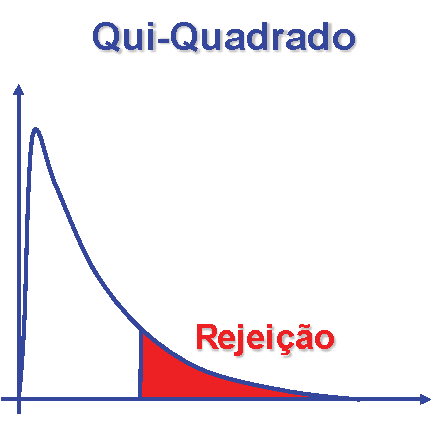
\includegraphics[width=0.46\textwidth]{Textuais/Figuras/qui-quadrado.pdf}
    \fonte{Autores}
    \label{fig:qui-quadrado}
\end{figure}

\subsection{Kolmogorov-Smirnov}

Esse teste é aplicado para verificar se os valores de uma certa amostra de dados podem ser considerados de uma população, com distribuição teórica pré-estabelecida.
O teste relaciona duas distribuições de frequências acumuladas, uma F’(x) teórica e outra F(x) derivada dos dados amostrais. O valor de $D_{max}$ dado pela Equação \ref{eq:kolmogorov}.

\begin{equation}
\label{eq:kolmogorov}
    D_{Max} = Max|F'(x) - F(x)|
\end{equation}

Caso o valor do $D_{max}$ observado seja inferior ao $D_{max}$ obtido em tabelas, a um determinado nível de significância $\alpha$, a hipótese de nulidade não é rejeitada, dessa forma, pode-se afirmar que os dados amostrais tem aderência à distribuição teórica.

O teste de Kolmogorov-Smirnov é muito utilizado em hidrologia, apesar de ser menos geral que outros testes, como o $\chi^2$, pois é aplicável apenas para testar a adequação do ajuste de distribuições contínuas, completamente especificados, isto é, quando não existem parâmetros a serem determinados \cite{hidrologia-estatistica-np}.

De acordo com \citeonline{estatistica-siegel}, o teste de Kolmogov-Smirnov procura especificar a distribuição de frequência acumulada teórica que ocorreria sob a distribuição de frequência acumulada observada. Determina-se o ponto em que essas duas distribuições – teórica e observada – acusam maior divergência. A referida distribuição amostral indica se essa diferença máxima pode ser atribuída ao acaso, ou seja, se uma divergência com tal magnitude teria probabilidade de ocorrer se as observações constituíssem realmente uma amostra aleatória da distribuição teórica. 

\begin{figure}[h]
    \caption{Análise das divergências do teste KS entre pontos amostrais e uma distribuição adotada}
    \centering
    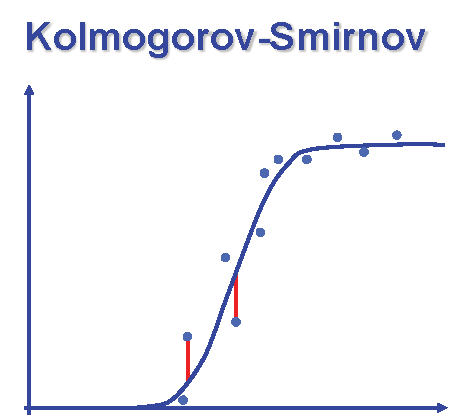
\includegraphics[width=0.5\textwidth]{Textuais/Figuras/kolmogorov.pdf}
    \fonte{Autores}
    \label{fig:kolmogorov}
\end{figure}